% !TEX root = ../main.tex
%-------------------------------------------------------------------------------
%-------------------------------------------------------------------------------
\begin{frame} I draw on the material presented in:\vspace{0.3cm}

\begin{itemize}\setlength\itemsep{1em}
  \item \bibentry{Gorelick.2014}
  \item \bibentry{Lanaro.2017}
\end{itemize}

\end{frame}%-------------------------------------------------------------------------------
%-------------------------------------------------------------------------------
\begin{frame}\textbf{Profiling}\vspace{0.3cm}

\begin{itemize}\setlength\itemsep{1em}
    \item \textit{Premature optimization is the root of all evil.}
    \item focus on readability
    \item set up development environment
    \item flesh out testing harness
    \item tackle performance bottlenecks
\end{itemize}

\end{frame}
%-------------------------------------------------------------------------------
%-------------------------------------------------------------------------------
\begin{frame}\textbf{Points of attack}\vspace{0.3cm}

\begin{itemize}\setlength\itemsep{1em}
    \item pure Python
    \item high-performance libraries, SciPy Stack
    \item compilation to faster language
    \item parallel processing
    \item distributed computing
\end{itemize}

\end{frame}
%-------------------------------------------------------------------------------
%-------------------------------------------------------------------------------
\begin{frame}
	\begin{figure}[htp]\centering
    \scalebox{0.3}{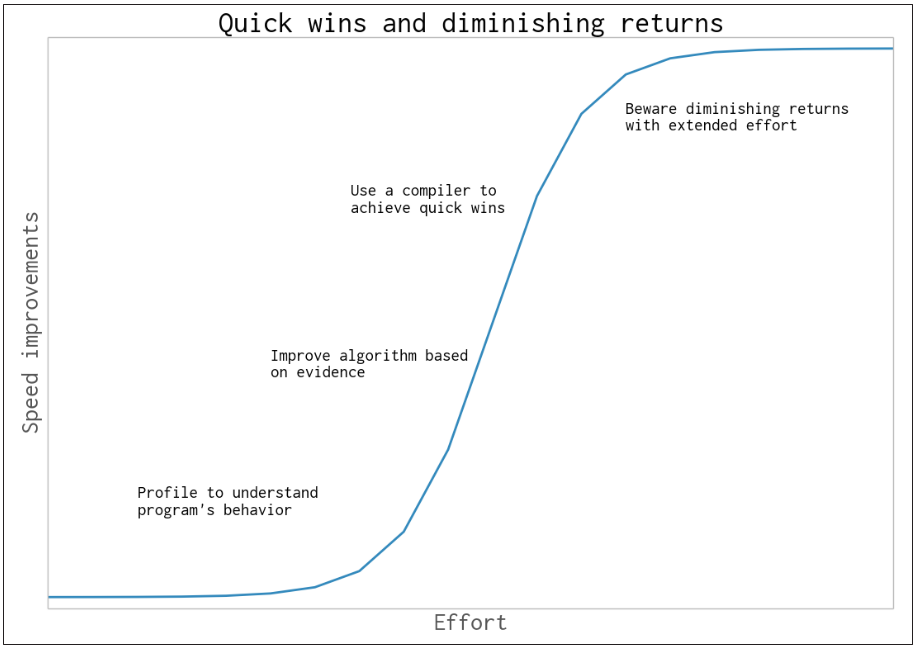
\includegraphics{fig-diminishing-returns}}
	\end{figure}
\end{frame}
